%--------------------------------------------------------------------------------------------------
% ips-phd-thesis-eng-apa.tex v1.3 (see the end of the file for modification history)
% To be used with ipsthesis.cls v1.3
% 
% A template for creating a PhD thesis in English using the APA 6th edition reference formatting
% with several accompanying files.  
% By Tea Tušar <tea.tusar@ijs.si>
%
% IMPORTANT NOTE: Biber must be used as the backhand for processing bibliographies, not bibtex!
%
% To compile this template, you need to run the following sequence of commands:
% 1. pdflatex  ips-phd-thesis-eng-apa
% 2. biber     ips-phd-thesis-eng-apa
% 3. makeindex ips-phd-thesis-eng-apa (optional, if you want an index)
% 4. pdflatex  ips-phd-thesis-eng-apa 
% 5. pdflatex  ips-phd-thesis-eng-apa
%--------------------------------------------------------------------------------------------------
\documentclass[phd,eng,apa]{ipsthesis}

\usepackage{amsmath}
\usepackage{amsfonts}
\usepackage{float}
\usepackage{tablefootnote}
\usepackage[utf8]{inputenc}
\usepackage{caption}
\usepackage{makecell}

\DeclareMathSymbol{\mhyphen}{\mathord}{AMSa}{"39}

%
%--------------------------------------------------------------------------------------------------
%  
% PREAMBULE
%--------------------------------------------------------------------------------------------------
%
% Files with bibliographies 
\addbibresource{references.bib}
%
% Define here all other packages and commands you need for your thesis, for example:
\usepackage{color}
\usepackage{listings}
\usepackage{longtable}
%--
% MP added for comments
\usepackage{todonotes}
%--------------------------------------------------------------------------------------------------
%  
% DOCUMENT
%--------------------------------------------------------------------------------------------------
\begin{document}
%--------------------------------------------------------------------------------------------------
%
% The cover page and spine are created separately using two .doc files provided by IPS.
%--------------------------------------------------------------------------------------------------
%
% FRONT MATTER
%--------------------------------------------------------------------------------------------------
%
\frontmatter
%
\selectlanguage{american}
\pagestyle{fancy}
%
% Title pages
%--------------------------------------------------------------------------------------------------
% 
% INPUT FOR THE TITLE PAGES
%--------------------------------------------------------------------------------------------------
% 
% Author
\author{Nikola Ivačič}         
%
% Title in English (use \protect\\ instead of \\ to create a line break)
\titleEnglish{Retrieval Augmented Multilingual Multi-label Text Classification for Low-resourced Languages and Environments}
%
% Supervisor (title and name, affiliation)
\supervisorOne{Prof.\ Dr. Nada Lavrač}{Jožef Stefan International Postgraduate School, Ljubljana, Slovenia}
%
% Co-supervisor (title and name, affiliation), optional
\supervisorTwo{Prof.\ Dr. Matthew Purver}{School of Electronic Engineering and Computer Science, Queen Mary University of London, London, UK}
%
% 
% Date
\thesismonth{September}
\thesisyear{2024}
%
\maketitle 
% 
% English abstract
%--------------------------------------------------------------------------------------------------
% 
\chapter*{Abstract}
\pdfbookmark[0]{Abstract}{Abstract}
%--------------------------------------------------------------------------------------------------
The recent development of large language models (LLMs) has significantly advanced the field of Natural Language Processing (NLP) and taken a leading role in the development of Artificial Intelligence.
We can see that trends are shifting not only towards extremely large models with multiple modalities and massive numbers of parameters but also towards smaller models that can be deployed outside large datacenter clusters.
However, smaller LLMs are still predominantly based on the English language and have rarely been pre-trained on lesser-used, low-resource languages.
Therefore, the model size and multilinguality still present a substantial obstacle to using state-of-the-art LLMs in specific industries, where low latency, high data volumes, autonomy, and resistance to outages are crucial.

In this paper, we analyze possible approaches to multi-label text classification (MTLC) for a specific media monitoring dataset that includes low-resourced languages and a large number of labels.
We propose a novel MTLC method that addresses the challenges of multi-linguality, low latency, model size, and label count based on concepts similar to Retrieval Augmented Generation (RAG) but used in the context of MTLC.
Due to the extremely fast pace of research and development in the field of NLP, we tried to employ a method agnostic to a specific LLM model selection, which wouldn't need constant fine-tuning because of frequent label changes.
This method could also provide a basis for further development of multipurpose systems, including online clustering and summarization for the media monitoring industry.

%
% Contents
\maketoc
%
%--------------------------------------------------------------------------------------------------
%
% MAIN MATTER
%--------------------------------------------------------------------------------------------------
%
\mainmatter
\captionsetup{font=small}
%
%--------------------------------------------------------------------------------------------------
% 
\chapter{Introduction}
%--------------------------------------------------------------------------------------------------
In this section, we delve into specific industries' challenges, focusing on applying deep-learning solutions to the multi-label text classification (MLTC) problem. We will examine the latest trends in Natural Language Processing (NLP) development and provide an overview of the foundational concepts that underpin our approach.

\section{Media Monitoring Industry}
Initially, the primary goal of media monitoring and analysis was to alleviate the burden of manually tracking all published news. However, as the news volume surged, the field had to evolve, incorporating more sophisticated NLP techniques. Media monitoring and analysis hold significant potential for societal benefit because they aim to present and scrutinize news content impartially without favouring any particular viewpoint. Furthermore, these processes help society by identifying biased perspectives, misinformation, and sentiment within news content.

In today's fast-paced world, media monitoring and analysis require near real-time capabilities to deliver timely and relevant information. This process involves categorizing articles by content, attaching metadata tags, and synthesizing information from multiple news sources. Advanced NLP techniques are well-suited to these tasks, enabling the development of personalized news recommendation systems, automated content summarization, and effective organization and prioritization of news items. Furthermore, the industry demands systems that ensure low-latency processing and operate autonomously, without relying on third-party services, to maintain data integrity, security, and uninterrupted access to critical updates.

Intense competition has significantly reduced profit margins in the media monitoring industry, particularly in the Western Balkan region. 
This financial pressure limits the ability to invest in large-scale hardware necessary for deploying state-of-the-art NLP technology in server clusters. 
Consequently, we are focusing on researching solutions that can efficiently run on consumer-grade hardware, enabling low-resource and cost-effective operations without sacrificing performance.

We aim to tackle the specific challenge of classifying news articles in South Slavic languages with custom-tailored topics for end users. 
For this purpose, we developed a new $NewsMon$ dataset, which involved sampling, preparing, and analyzing a collection of labelled news articles sourced from the news monitoring industry. 
This dataset contains over a million articles and more than twelve thousand labels for the classifier to learn, placing this challenging classification task in the realm of large-scale if not extreme, multilabel classification.

Similar challenges, such as assigning a few labels from a vast label space, also arise in other industries, like tagging keywords for online shopping items or classifying industrial products for tax purposes~\parencite{zhang2023longtailed}.

\section{Pretrained Large Language Models}
\label{sec:llm}
In Natural Language Processing, Transformer-based deep neural network models~\parencite{vaswani2017attention} have recently become the leading approach. 
While Transformer Encoder architecture initially drove the transition to the usage of pre-trained large language models like BERT~\parencite{devlin2018bert} and RoBERTa~\parencite{liu2019roberta}, the most significant advancements have occurred with generative, text-to-text Transformer models. 
Notable examples include complete Transformer architecture models like T5~\parencite{raffel2020exploring} and popular Auto-Regressive Transformer Decoder architectures such as the GPT family~\parencite{radford2018improving, radford2019language, brown2020language}, LaMDA~\parencite{thoppilan2022lamda}, PaLM~\parencite{chowdhery2022palm}, and LLaMA~\parencite{touvron2023llama, touvron2023llama2openfoundation}. 
These models are pre-trained on extensive text datasets and fine-tuned for various text-based tasks, including question-answering, text generation, and language translation, significantly advancing language understanding and generation capabilities. 
The top-performing MLTC systems also utilize Transformer-based deep neural network models~\parencite{tarekegn2024deeplearningmultilabellearning}.

Current trends in Large Language Models (LLMs) evolve along two distinct yet complementary paths. 
On the one hand, we're witnessing the development of increasingly sophisticated and performant families of models characterized by massive training datasets, enormous parameter counts, multi-modal capabilities~\parencite{openai2024gpt4technicalreport, dubey2024llama3herdmodels, geminiteam2024geminifamilyhighlycapable} and substantial compute and energy cost~\parencite{rae2021scaling, thoppilan2022lamda}.
These versatile Foundation Models have state-of-the-art capabilities for text classification but are out of reach, given our initial constraints.
However, there is a significant opportunity to use these models to generate synthetic training data for fine-tuning smaller, more efficient models~\parencite{kuzman2023chatgptbeginningendmanual}.
On the other hand, there's a growing focus on developing smaller, more efficient language models that can run on less powerful hardware~\parencite{li2024DataCompLM, gemma_2024, abdin2024phi3technicalreporthighly, jiang2023mistral7b, parmar2024nemotron415btechnicalreport}. 
This trend aims to bring the power of advanced language processing to edge devices, enabling real-time, on-device inference without relying on third-party cloud infrastructure. 

Unfortunately, these smaller, efficient language models largely lack pre-training in South Slavic languages. 
They cannot operate on consumer-grade hardware without techniques like pruning, knowledge distillation~\parencite{muralidharan2024compact, hinton2015distillingknowledgeneuralnetwork, gu2024minillmknowledgedistillationlarge} or quantization~\parencite{nagel2021whitepaperneuralnetwork, gholami2021surveyquantizationmethodsefficient, malinovskii2024pvtuningstraightthroughestimationextreme}, and they often come with restrictive licensing terms for industrial use. 
Additionally, deploying these models in a production environment may lead to significant inference latency, causing critical delays.

\section{Retrieval Augmented Approaches}

Retrieval-Augmented Generation (RAG) is an innovative technique in natural language processing that enhances pre-trained language model text generation by incorporating external knowledge sources~\parencite{lewis2021retrievalaugmentedgenerationknowledgeintensivenlp}. 
By combining these strengths, RAG excels in knowledge-intensive NLP tasks, where ensuring factual accuracy and delivering up-to-date information is critical. 
This approach allows models to dynamically retrieve relevant data, significantly improving their performance in complex applications. 
RAG models consist of four main components: 
\begin{itemize}
    \item Encoder: Commonly, a language model, fine-tuned on retrieval tasks, is used to obtain the dense query and text passage representation.
    \item Document Index: On disk or in memory document index or a database containing dense document or text passage representation.
    \item Retriever: Typically a Dense Passage Retriever (DPR) that fetches relevant document passages from a large corpus~\parencite{karpukhin2020dense}
    \item Generator: Usually a pre-trained sequence-to-sequence model like Auto-Regressive Transformer Decoder (see section~\ref{sec:llm}) for answering or summarisation based on a context from retrieved passages.
\end{itemize}

Our approach draws inspiration from this work, particularly by integrating pre-trained Transformer Encoder models with non-parametric memory using a general-purpose fine-tuning method and a dense retriever.
In our scenario, using non-parametric memory and a dense retriever minimizes the need for continuous model fine-tuning, as labels are frequently updated, added and removed. 

We can find a similar approach in the work of \textcite{zhang2023longtailed}, which addresses extreme multi-label text classification (XMTC) with a novel framework of Dual Encoder with Pseudo Label (DEPL).
DEPL treats each input document as a query, utilizing a neural network model to retrieve relevant labels from the candidate space based on their textual descriptions. 
To achieve this, a linear support vector machine (SVM) model is trained using bag-of-words (BoW) features, such as TF-IDF, to generate informative keywords automatically. 
These keywords serve as pseudo descriptions for each label, helping the model accurately identify and match the appropriate labels for each document.

\section{Scope and Objectives}
This paper presents the analysis of the news monitoring data collected for our research. 
By examining the current state-of-the-art in MTLC and XMTC, we aim to compare and identify potential improvements to our information retrieval method. 
Finally, we present the foundations of our approach and share the results of our initial experiments.

\section{Organization of the Paper}

%The following chapter introduces the data, explains how it was created, and compares it to a similar, well-studied dataset. 
%We then explore the evaluation metrics for MTLC and XMTC, followed by an analysis of the latest advancements in the field and their contributions in Chapter~\ref{ch:background}.
%Next, in Chapter~\ref{ch:retrieval}, we present our method, baseline models, and a preliminary zero-shot evaluation. 
%In the final Chapter~\ref{ch:trends}, we discuss potential enhancements and outline our planned research efforts for the future.

The following chapter introduces the background of our research. 
We explore the evaluation metrics for MTLC and XMTC and then analyze the latest advancements in the field and their contributions.
We then introduce the data, explain its creation, and compare it to a similar, well-studied dataset in Chapter~\ref{ch:data}.
Next, in Chapter~\ref{ch:retrieval}, we present our method, embedding models, baseline and preliminary zero-shot experiments.
In the final Chapter~\ref{ch:trends}, we discuss potential enhancements and outline our planned research efforts for the future.

%--------------------------------------------------------------------------------------------------
% 
\chapter{Background}
\label{ch:background}
%--------------------------------------------------------------------------------------------------
Recently, transformer-based models have emerged as the leading performers in multi-label text classification (MLTC), as highlighted by ~\textcite{tarekegn2024deeplearningmultilabellearning}. 
Despite some models achieving high performance without the use of pre-trained language models, as noted by ~\textcite{duan2022fusiontwostream, liu2022cnle}, methods utilizing language pretraining, such as those discussed by~\textcite{yarullin2020bertforseq, fallah2023exploitinglabeldependencies, li2024kenet}, consistently outperform others. 
Most of the revised methods use these models to obtain a dense document representation, a cornerstone of MLTC.
A significant challenge with these pre-trained models is their limitation on text length, which impacts up to 50\% of the instances in our dataset, as illustrated in Figure~\ref{fig:tokens_hist}.

\begin{figure}[h!]
  \centering
  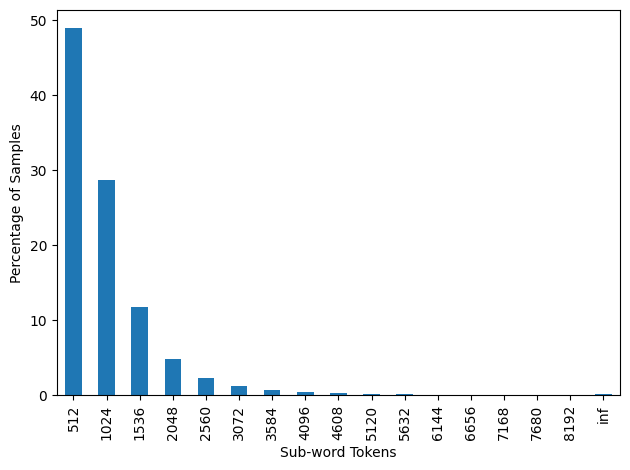
\includegraphics[width=0.6\textwidth]{figures/tokens_hist.png}
  \caption{The distribution of \textit{SentencePiece} sub-word tokens in the $NewsMon$ dataset.}
  \label{fig:tokens_hist}
\end{figure}

Transitioning from standard multi-label text classification to large-scale scenarios shifts the evaluation metrics used, complicating the comparison of different approaches. 
Precision, recall, and F1-score metrics are standard in a typical multi-label setting. 
However, as the scale increases and datasets grow more complex with numerous labels, these metrics might not adequately capture performance nuances.

Extreme and Large-scale classification often incorporates metrics like mean average precision, nDCG (Normalized Discounted Cumulative Gain), and precision at K, considering the ranking of predictions and the relevance of top K labels. 
These metrics are sensitive to the order of labels and the depth of relevance, which are less emphasized in smaller-scale settings.
This metric shift reflects the increased complexity and different priorities in large-scale systems, such as the importance of retrieving the most relevant labels from a vast set. 
% Co-attention network with label embedding for text classification - Co-attention Network with Label Embedding (CNLE)
% Exploiting Label Dependencies for Multi-Label Document Classification Using Transformers - Loss Function adaptation
% Kenet: Knowledge-Enhanced DOC-Label Attention Network for Multi-Label Text Classification

To address this and other challenges, this chapter will first outline the evaluation metrics commonly used in MLTC, focusing on those developed for large-scale multi-label research~\parencite{bhatia2016extremerepo} originating from the field of Information Retrieval (IR)~\parencite{manning2008}. 
Subsequently, we will delve into methods designed to manage text truncation issues inherent in pre-trained language models. 
Finally, we will explore advanced techniques from the most effective MLTC approaches that could potentially refine our methodology and improve performance.

\section{Evaluation Metrics}
Following the work of ~\textcite{tsoumakas2010, madjarov2012, tarekegn2024deeplearningmultilabellearning} and many more, we can observe that all of the well-known classification metrics are used for MLTC research.
While micro averaged $F_1\mhyphen score$ and a $Hamming\mhyphen Loss$ are the most popular in MLTC, they are usually not considered in extreme multi-label text classification (XMTC) research.
In the case of XMTC, the rank-based IR metrics are considered~\parencite{manning2008, bhatia2016extremerepo, chalkidis-etal-2019-large, you2019attentionxmllabeltreebasedattentionaware, chang2020tamingpretrainedtransformersextreme, zhang2023longtailed}.
Therefore, we present three categories of metrics:
\begin{itemize}\itemsep=0pt
    \item Example-based metrics, namely $Hamming\mhyphen Loss$ and $Accuracy$, to assess the differences between the actual and predicted label sets across all instances.
    \item Label-based metrics, including $Precision$, $Recall$, and $F_1\mhyphen score$, to examine performance averaged across all labels.
    \item Rank-based metrics, including $P@K$, $R@K$, $R-precision@K$, and $nDCG@K$
\end{itemize}

In this section, we use $N$ for the number of instances, $L$ for the number of labels, $y_i$ for an individual example label set, and $\hat{y_i}$ for the predicted example label set.

\subsection{Example-based metrics}
For the example-based evaluation, we usually consider
\begin{itemize}
  \item Subset accuracy:
    \begin{equation}
      Accuracy = \frac{1}{N}\sum_{i=1}^{N}I( y_i = \hat{y_i})
    \end{equation}
    where  $I(true) = 1$ and $I(false) = 0$
  \item Hamming loss:
    \begin{equation}
      Hamming\mhyphen Loss = \frac{1}{N \cdot L}\sum_{i=1}^{N}\sum_{j=1}^{L}{xor(y_{i_j},\hat{y_{i_j}})}
    \end{equation}
\end{itemize}
Contrary to Subset accuracy, a Hamming loss closer to 0 means a better score.
\begin{table}[htb]
    \caption{Example $Hamming\mhyphen Loss$ calculation: $\frac{5}{4 \cdot 5} = 0.25$ where each row contains a target $y_i$ followed by a prediction $\hat{y_i}$ vector with five label values with five wrong predictions in total.}
	\label{tab:hamming}
	\centering
    \begin{tabular}{lll}
        \hline
        &$y_i$&$\hat{y_i}$\\
        \hline
        $x_1$&$[1, 0, 1, 1, 0]$&$[1, 0, 1, \textcolor{red}{0}, \textcolor{red}{1}]$\\
        $x_2$&$[0, 1, 1, 0, 0]$&$[0, 1, 1, \textcolor{red}{1}, 1]$\\
        $x_3$&$[0, 0, 0, 1, 0]$&$[0, 0, \textcolor{red}{1}, 1, \textcolor{red}{1}]$\\
        $x_4$&$[1, 1, 0, 1, 0]$&$[1, 1, 0, 1, 0]$\\
        \hline
    \end{tabular}
\end{table}

With a large label set characterized by a long-tail distribution and minimal label density, both Subset accuracy and Hamming loss metrics tend to be very small.
Subset Accuracy tends to be small because such datasets usually have high label diversity versus cardinality; hence, it is hard to predict rare combinations exactly.
Hamming loss is typically very low, which is a desired property. Still, it is low due to the small label cardinality relative to the total number of labels, even when the model performs poorly.

\subsection{Label-based metrics}
For the label-based evaluation, we define:
\begin{itemize}
  \item Micro-averaged Precision and Recall:
    \begin{equation}
      Precision_{micro} = \frac{\sum_{i=1}^{L} TP_i}{\sum_{i=1}^{L} (TP_i + FP_i)}
    \end{equation}
    \begin{equation}
      Recall_{micro} = \frac{\sum_{i=1}^{L} TP_i}{\sum_{i=1}^{L} (TP_i + FN_i)}
    \end{equation}
  \item Macro-averaged Precision and Recall:
    \begin{equation}
      Precision_{macro} = \frac{1}{L}\sum_{i=1}^{L}\frac{TP_i}{TP_i + FP_i}
    \end{equation}
    \begin{equation}
      Recall_{macro} = \frac{1}{L}\sum_{i=1}^{L}\frac{TP_i}{TP_i + FN_i}
    \end{equation}
\end{itemize}
given that:
\begin{itemize}\itemsep=0pt
  \item False Positives (FP): a class or label predicted but not present in the test.
  \item False Negatives (FN): a class or label is present in the test but missing in our prediction.
  \item True Positives (TP): a class or label that is correctly predicted.
  \item True Negatives (TN): a class or label that is correctly not predicted and not present in the test.
\end{itemize}
Precision measures the accuracy of positive predictions, and Recall (also known as sensitivity) measures a classifier's ability to find all relevant instances in a dataset.
In both cases, the harmonic mean of precision and recall, the $F_1\mhyphen score$, can be computed as follows:
\begin{equation}
  F_1\mhyphen score = 2  \cdot \frac{Precision \cdot Recall}{Precision +  Recall}
\end{equation}
% Micro-averaging is more widely used than macro-averaging for MTLC model evaluation. Hmnn

\subsection{Ranking-based metrics}
Common evaluation measures for Large-scale Multi-Label Text Classification (LMTC) include precision (P@K) and recall (R@K) for the top K predicted labels, averaged over test samples:

\begin{equation}
P@K = \frac{1}{N} \sum_{i=1}^N \frac{S_i(K)}{K}
\end{equation}
\begin{equation}
R@K = \frac{1}{N} \sum_{i=1}^N \frac{S_i(K)}{R_i}
\end{equation}

where $K$ is the number of labels to be selected per instance, $N$ is the total number of test instances, $S_i(K)$ is the number of correct labels among those ranked as top $K$ for the i-th instance, and $R_i$ is the number of gold labels for each instance.
Although these measures are widely used in LMTC, \textcite{chalkidis-etal-2019-large} questions their appropriateness for the following reasons:
\begin{itemize}
    \item $R@K$ leads to excessive penalization when instances have more than K gold labels. 
    For example, evaluating at $K = 1$ for a single document with five gold labels returns $R@1 = 0.20$ if the system returns a correct label. 
    The system is penalized even though it cannot return more than one label.
    \item $P@K$ does the same for instances with fewer than $K$ gold labels. 
    For example, evaluating at $K = 5$ for a single document with a single gold label returns $P@1 = 0.20$.
\end{itemize}

Both measures tend to overestimate or underestimate performance on documents where the number of gold labels significantly deviates from $K$.
Due to these limitations, these metrics fail to accurately identify the most effective methods.

Given the issues mentioned, \textcite{chalkidis-etal-2019-large} argues that $R\mhyphen Precision@K$ and $nDCG@K$ offer a more informative and equitable evaluation. These measures adapt to the actual number of gold labels per instance, providing a more accurate performance assessment regardless of whether instances have few or many gold labels. We define the macro-averaged versions of these two measures as follows:
\begin{itemize}
    \item Macro-averaged $R\mhyphen Precision@K$:
        \begin{equation}
        R\mhyphen Precision@K = \frac{1}{N} \sum_{i=1}^N \frac{S_i(K)}{\min(K, R_i)}
        \end{equation}
    This measure is the same as $P@K$ if there are at least $K$ gold labels; otherwise, $K$ is reduced to the number of gold labels.
    For large values of $K$ that tend to exceed the number of gold labels, $R\mhyphen Precision@K$ asymptotically approaches $R@K$.
    \item Macro-averaged $nDCG@K$ (normalized discounted cumulative gain):
        %\begin{equation}
        %nDCG@K = \frac{1}{N} \sum_{i=1}^N \sum_{j=1}^K \frac{2^{S_i(j)} - 1}{log_2(1 + j)}
        %\end{equation}
        In general, we define for each instance:
        \begin{equation}
        DCG@K = \sum_{j=1}^K \frac{gain_j}{discount_j} = \sum_{j=1}^K \frac{2^{S_i(j)} - 1}{log_2(j + 1)}
        \end{equation}
        and normalize it by ideal $IDCG@K$ or maximum $DCG@K$ computed from ground truth labels:
        \begin{equation}
        nDCG@K = \frac{DCG@K}{IDCG@K}
        \end{equation}
        Since there is no ordering of labels in the ground truth in the multi-label case, the equations can be slightly rewritten as:
        \begin{equation}
            \text{DCG}@k := \sum_{l\in {\text{rank}}_k (\hat{\mathbf y})} \frac{\mathbf y_l}{\log(l+1)}
        \end{equation}
        Where $\hat{\mathbf y} \in {\mathbb{R}}^{L}$ is a predicted score vector, $\mathbf y \in \left\lbrace 0, 1 \right\rbrace^L$ is a ground truth label vector, $\text{rank}_k(\mathbf y)$ returns the $k$ largest indices of $y$ ranked in descending order~\parencite{bhatia2016extremerepo}.
        \begin{equation}
            \text{nDCG}@k := \frac{{\text{DCG}}@k}{\sum_{l=1}^{\min(k, \|\mathbf y\|_0)} \frac{1}{\log(l+1)}},
        \end{equation}
        Finally, we define micro-averaged value as:
        \begin{equation}
        nDCG@K = \frac{1}{N} \sum_{i=1}^N nDCG@K_i
        \end{equation}
\end{itemize}

\section{Long Document Representation}
\label{sec:long_doc}

The shift from classifying short to long documents presents significant challenges. BERT~\parencite{devlin2018bert}, RoBERTa~\parencite{liu2019roberta}, XLM-RoBBERTa~\parencite{conneau2019xlmr} and many related models are pre-trained on sequences of up to 512 tokens, which can not be considered a long document. A typical method involves truncating longer documents to the first 512 tokens, enabling the direct use of these pre-trained models. 
However, truncating text can exclude critical information; therefore, we believe this approach is insufficient for long document classification. 
This can negatively affect the classification performance. 
Another significant challenge is the computational and memory overhead associated with the vanilla Transformer architecture's $O(n^2)$ complexity, which prevented using longer contexts before the LLM era.

Early approaches were based on sparse self-attention instead of full-self attention (Longformer; \textcite{beltagy2020longformerlongdocumenttransformer},  and Big Bird; \textcite{zaheer2021bigbird}), dividing long documents into smaller chunks (Hierarchical Transformers; \textcite{pappagari2019hierarchical}), or using only selected sentences from the document that are salient to making the classification decision (CogLTX; \textcite{ding2020cogltx}).

\begin{table}[H]
	\centering
    \resizebox{\textwidth}{!}{%
        \begin{tabular}{lccccccc}
        \hline
        \textbf{Dataset} & \textbf{Type} & \textbf{\# Train} & \textbf{\# Dev} & \textbf{\# Test} & \textbf{\# Labels} & \textbf{\# BERT Tokens} & \textbf{\% Long} \\
        \hline
        Hyperpartisan & binary & 516 & 64 & 65 & 2 & 744.18 ± 677.87 & 53.49 \\
        20NewsGroups & multi-class & 10,182 & 1,132 & 7,332 & 20 & 368.83 ± 778.34 & 11.30 \\
        EURLEX57K & multi-label & 45,000 & 6,000 & 6,000 & 4,271 & 707.99 ± 538.69 & 51.30 \\
        Inverted & multi-label & 10,230 & 1,279 & 1,279 & 227 & 574.31 ± 659.56 & 38.76 \\
        Book Summary & multi-label & 5,115 & 639 & 639 & 227 & 1,148.62 ± 933.97 & 75.54 \\
        \hline
        \end{tabular}
    }
\caption{Statistics on the datasets. \# BERT Tokens refers to the average token count obtained via the tokenizer of the BERT base model (uncased). \% Long refers to the percentage of documents with more than 512 BERT tokens~\parencite{park2022efficient}.}
\label{tab:park_dataset}
\end{table}

\begin{table}[H]
	\centering
    \resizebox{\textwidth}{!}{%
        \begin{tabular}{lcccccc}
        \hline
        \rule{0pt}{4ex} \textbf{Model} & \textbf{Hyperpartisan} & \textbf{20NewsGroups} & \textbf{EURLEX} & \rule[-2ex]{0pt}{0pt} \parbox[c]{2cm}{\textbf{Inverted\newline EURLEX}} & \parbox[c]{2cm}{\textbf{Book\newline Summary}} & \parbox[c]{2cm}{\textbf{Paired\newline Summary}} \\
        \hline
        BERT & 88.00 & \underline{86.09} & \underline{66.76} & 62.88 & 60.56 & 52.23 \\
        BERT+TextRank & 85.63 & 85.55 & 66.56 & \underline{64.22} & 61.76 & 56.24 \\
        BERT+Random & 83.50 & \textbf{86.18} & \textbf{67.03} & \textbf{64.31} & \textbf{62.34} & 56.77 \\
        Longformer & \textbf{93.17} & 85.50 & 44.66 & 47.00 & 59.00 & \textbf{58.85} \\
        ToBERT & 86.50 & -- & 61.85 & 59.50 & 61.38 & \underline{58.17} \\
        CogLTX & \underline{91.91} & 86.07 & 61.95 & 63.00 & 60.71 & 55.74 \\
        \hline
        \end{tabular}
    }
\caption{Performance metrics evaluated on long documents in the test set for all datasets. The average accuracy (\%) over five runs is reported for Hyperpartisan and 20NewsGroups, while the average micro-F1 (\%) is used for the other datasets. The highest value per column is in bold, and the second highest value is underlined~\parencite{park2022efficient}.}
\label{tab:park_longdoc}
\end{table}

\textcite{park2022efficient} argues that the effectiveness of various models remains ambiguous due to the absence of a unified consensus on benchmark datasets and established baselines. 
Often, new variants of efficient Transformers are only compared against a BERT/RoBERTa baseline, with limited comparisons to other Transformer models designed explicitly for the task~\parencite{beltagy2020longformerlongdocumenttransformer, zaheer2021bigbird}.
Conversely, models tailored for long document classification typically focus solely on comparing state-of-the-art models for specific datasets. 
They frequently overlook the inclusion of a BERT/RoBERTa baseline or comparisons~\parencite{pappagari2019hierarchical, ding2020cogltx}.



While \textcite{dai2022revisitingtransformer} research suggests that using Longformer or Hierarchical Transformers enhances performance in long document classification, \textcite{park2022efficient} and \textcite{jaiswal2023breakingtokenbarrierchunking} findings indicate the opposite, in the latter, vanilla BERT with 512 tokens extended random-sentence text block outperformed more advanced models (BERT and BERT-random CLS tokens were concatenated before the classification head, see Table~\ref{tab:park_longdoc}). 
Both studies demonstrate that the effectiveness of these models is highly dependent on the dataset used.
It is worth noting that all experiments were conducted using English-language pre-trained models and datasets.

\section{Extending the Position Encoding}
The development of pre-trained language models has driven innovations in text embedding techniques, including Sentence-BERT~\parencite{reimers-2019-sentence-bert} and SimCSE~\parencite{gao2022simcse}, which refine BERT by fine-tuning on natural language inference (NLI) datasets. 
To push the boundaries of text embedding performance and robustness, advanced methods and models designed for RAG and IR, like E5~\parencite{wang2024textembeddingsweaklysupervisedcontrastive} and BGE~\parencite{xiao2024cpackpackagedresourcesadvance} have been introduced. 
These methods implement a complex multi-stage training approach, beginning with pre-training on billions of weakly supervised text pairs and then fine-tuning on various high-quality labelled datasets. In both stages, contrastive learning plays a crucial role.
The process of contrastive learning involves selecting a random example as an anchor and then choosing positive and negative examples related to the anchor. 
Subsequently, positive examples are drawn closer to the anchor, while negative examples are pushed further away.

In recent years, reasonably sized models with impressive performance from this family have emerged, some even multilingual~\parencite{wang2024multilinguale5textembeddings}. 
However, many of these models are initialized from traditional pre-trained Transformer architectures and inherit their limitations, such as short context windows and, consequently, truncated text.
To address this issue, approaches have been developed to capture broader contexts and more comprehensive document semantics with modifications of positional encoding without the need to train the model from scratch.
\textcite{zhu2024longembedextendingembeddingmodels} provides a comprehensive \textit{LongEmbed} benchmark for both absolute positional and rotary positional encoding modifications to enable context window extension.
\begin{itemize}
    \item \textbf{Absolute Position Encoding (APE)} is the most common positional encoding technique used in models that follow the BERT architecture. In APE-based models, absolute position identifiers are converted into position vectors, which are then added to token embeddings. This combined input is subsequently processed through a series of transformer layers.
    \item \textbf{Rotary Position Encoding (RoPE)} is the most common position encoding strategy used in the era of LLMs, including LLaMA~\parencite{touvron2023llama}, Gemma~\parencite{gemma_2024}, Mistral~\parencite{jiang2023mistral7b}, etc. 
    It encodes position information of tokens with a rotation matrix that naturally incorporates explicit relative position dependency.
\end{itemize}
\textcite{zhu2024longembedextendingembeddingmodels} further categorizes the strategies for managing long input sequences in model processing:
\begin{enumerate}
    \item \textbf{Divide-and-Conquer:} This approach segments long inputs into shorter chunks, processes each individually, and then combines the results. This method is used in the PCW model \parencite{ratner2023parallelcontextwindowslarge}.
    \item \textbf{Position Reorganization:} This technique rearranges position identifiers to enhance the model's ability to handle longer sequences. Examples include SelfExtend \parencite{jin2024llmmaybelonglmselfextend} and DCA \parencite{an2024trainingfreelongcontextscalinglarge}, among others.
    \item \textbf{Position Interpolation:} This involves creating new position embeddings by interpolating between existing ones. Models employing this technique include PI \parencite{chen2023extendingcontextwindowlarge}, NTK \parencite{peng2023ntkaware}, YaRN \parencite{peng2023yarnefficientcontextwindow}, and Resonance RoPE \parencite{wang2024resonanceropeimprovingcontext}.
\end{enumerate}
Extending the Position Encoding allows for a more adequate representation of longer texts, enabling the retrieval system to consider the document as a whole rather than in fragmented parts.
While some of these methods can be used effectively on APE without additional fine-tuning (Parallel Context Windows, Grouped Positions, Recurrent Positions, Linear Position Interpolation), they generally yield better results when fine-tuned~\parencite{zhu2024longembedextendingembeddingmodels}.
There has been a noticeable trend in models designed for information retrieval (IR) that are initialized from large language models (LLMs), moving away from the previously predominant Transformer-Encoders.

\section{Recent MLTC and XMTC approaches}
In this section, we explore some of the recent state-of-the-art (SOTA) approaches in both Multi-Label Text Classification (MLTC) and Extreme Multi-Label Text Classification (XMTC), as datasets with similar sizes and properties appear in the research of both. 
Reviewing these methodologies, we aim to gain insights that could refine our approach.

We can split the document classification model into two parts: a document encoder that creates a dense document representation and a classifier that predicts one or multiple labels based on the encoded representation~\parencite{dai2022revisitingtransformer}. 

Multiple data labels often indicate relationships between different categories, leading recent methods to commonly address the issue of Label Dependency. 
In terms of modelling these dependencies, learning approaches are categorized into first-order (each label treated independently), second-order (modelling interactions between pairs of labels), and higher-order (addressing interactions among more than two labels simultaneously)~\parencite{tarekegn2024deeplearningmultilabellearning}.

Binary cross-entropy loss (BCE; \textcite{bengio2013bce}), when paired with a sigmoid activation function, is widely used in machine learning for addressing multi-label classification problems and can be considered a baseline loss function. 
With BCE, each label is considered an independent binary prediction.
The main challenge with BCE arises from the imbalance in label distribution and the complex dependencies among labels, which have inspired numerous studies on loss function design.
Focal loss (FL), introduced by \textcite{lin2017focal}, assigns greater weight to instances that are less likely to occur, which is interpreted as "harder to classify." 
Class-Balanced loss (CB), proposed by \textcite{cui2019classbalanced}, implements a re-weighting scheme upon FC based on the effective number of instances per class, reducing redundant information of head classes. 
Distribution-Balanced loss (DB) by \textcite{wu2020distributionbalanced} initially reduces redundant information resulting from label co-occurrence. Then, it incorporates Negative Tolerant Regularization (NTR) to reduce the weight of easy-to-classify negative labels.
Building on this, CB-NTR Loss by \textcite{huang2021balancing} combines the features of CB and NTR to better handle label imbalances and dependencies~\parencite{ma2023pai}.
A similar approach is taken by \textcite{fallah2023exploitinglabeldependencies}, which computes loss regularization term based on the dis-similarity vector - a result of the label co-occurrence matrix and the activations of the output layer of the classification.

In addition to incorporating label co-occurrence and imbalances into the loss function computation, contrastive learning techniques have become popular in some multi-label classification tasks~\parencite{piskorski-etal-2023-semeval-task3}.
For multi-label text classification, these methods often calculate a combined loss that includes both binary cross entropy and contrastive loss~\parencite{reiterhaas2023mcpt, liao2023marseclipse}.
Interestingly, we encountered similar techniques widely used in computer vision~\parencite{zheng-etal-2022-contrastive, tunstall2022efficient} as predominant in learning the dense document representations for IR and RAG systems in the previous Section~\ref{sec:long_doc}.

\begin{figure}[h!]
  \centering
  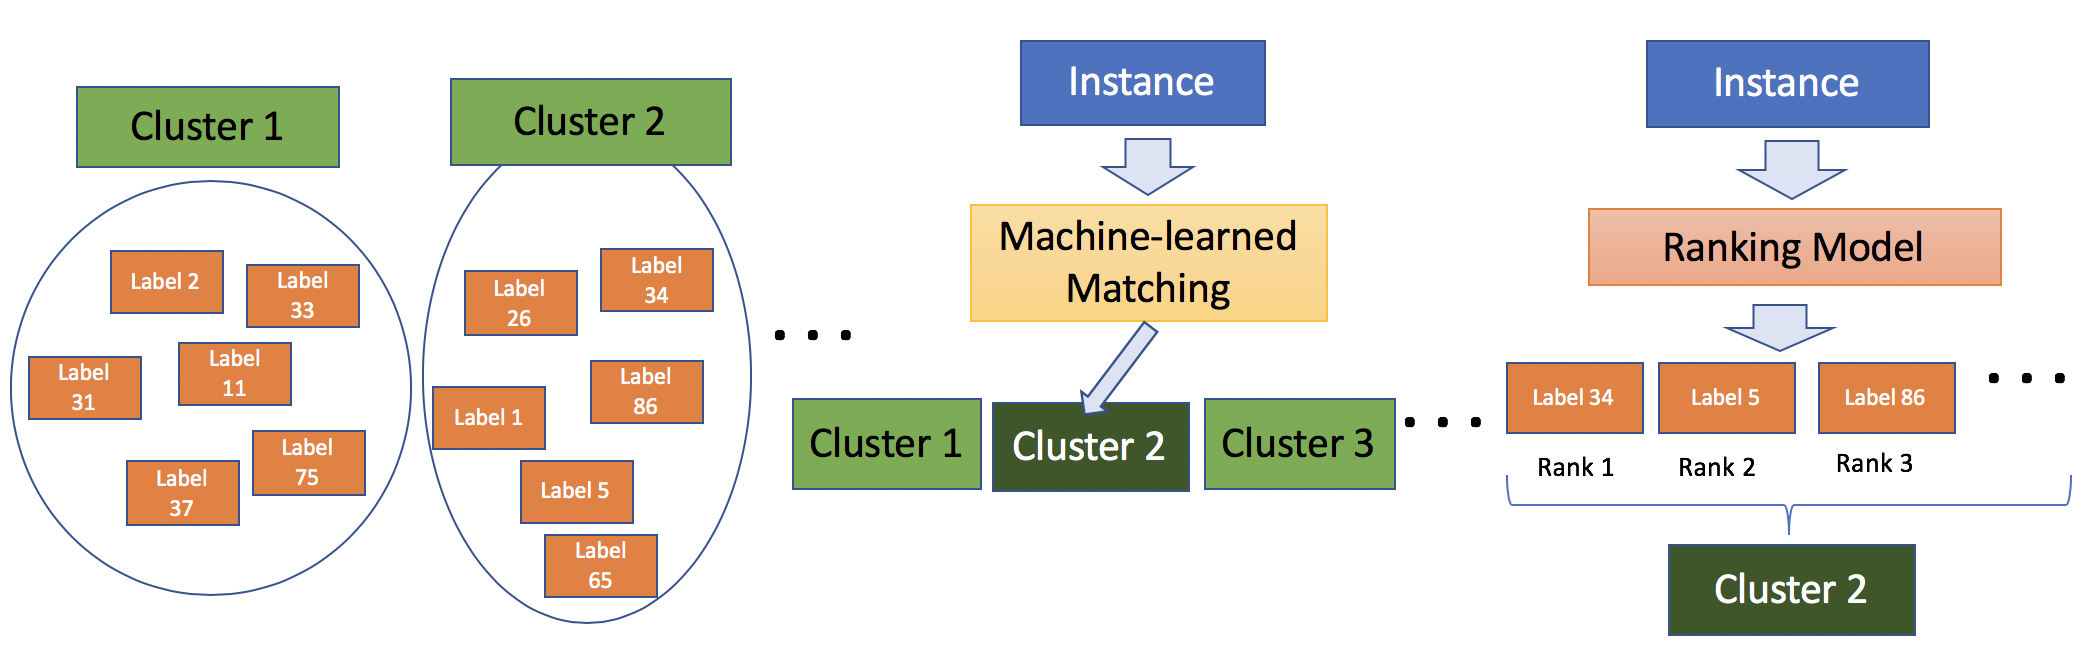
\includegraphics[width=0.9\textwidth]{figures/x-transformer_model.png}
  \caption{The proposed X-Transformer framework. First, Semantic Label Indexing reduces the large output space. Transformers are then fine-tuned on the XMTC sub-problem that maps instances to label clusters. Finally, linear rankers are trained conditionally on the clusters and Transformer’s output to re-rank the labels within the predicted clusters.~\parencite{chang2020tamingpretrainedtransformersextreme}.}
  \label{fig:x_trans_model}
\end{figure}

%TODO: in batch negative sampling popular in XMTC

Another class of approaches integrates label semantics directly into the neural network architecture by combining dense document representations with label representations. 
These methods differ in using either sparse or dense label representations and whether they employ the same or different encoders at various stages for labels and documents.
For example, in the domain of XMLC, sparse label representations are employed alongside Label Semantic Indexing to cluster labels and simplify the classification challenge with a large label count (see Figure\ref{fig:x_trans_model}). 

\begin{figure}[h!]
  \centering
  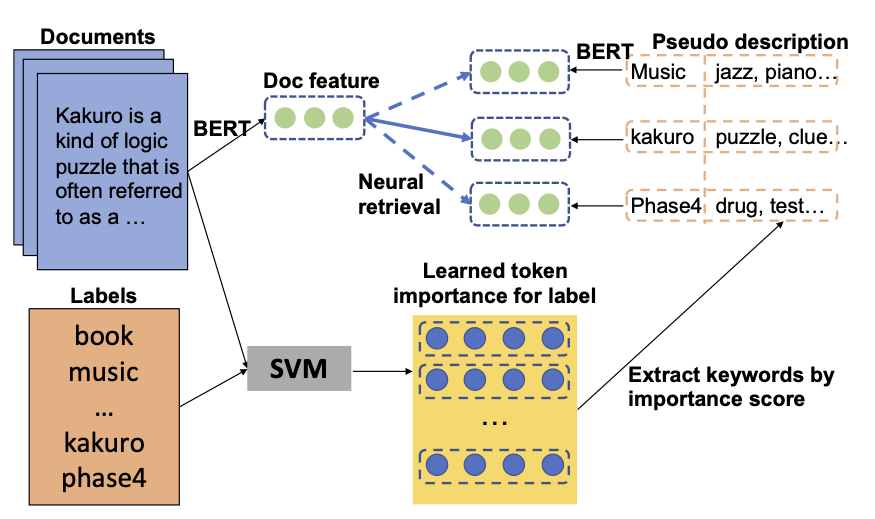
\includegraphics[width=0.5\textwidth]{figures/depl_model_2.png}
  \caption{The proposed DEPL framework. First, a BoW SVM classifier is trained, and top keywords from the label embeddings are extracted according to the importance of the learned token. 
  Then, keywords are concatenated with the original label names to form pseudo descriptions. 
  Finally, a neural retrieval model is leveraged to rank the labels according to semantic matching between document text and label descriptions~\parencite{zhang2023longtailed}.}
  \label{fig:depl_model}
\end{figure}

More recently, another method has improved the prediction of tail labels over the X-Transformer model. 
The DEPL model proposed by \textcite{zhang2023longtailed} uses sparse representations to augment labels with pseudo descriptions, which are then processed by the same encoder as documents. 
The SVM classification model is used to identify and concatenate the most important keywords related to each label, creating pseudo descriptions.
Specifically, they encode all the positive labels of the instances in the batch, add the top negative predictions from the sparse classifier, and include randomly sampled negatives to complete the batch. 
The loss is then calculated based on both positive and retrieved negative values during the training process (see Figure~\ref{fig:depl_model}).
This negative in-batch sampling technique is again similar to how other XMTC models~\parencite{jiang2021lightxmltransformerdynamicnegative} are trained and is inspired by IR models~\parencite{karpukhin2020dense}.

\begin{figure}[h!]
  \centering
  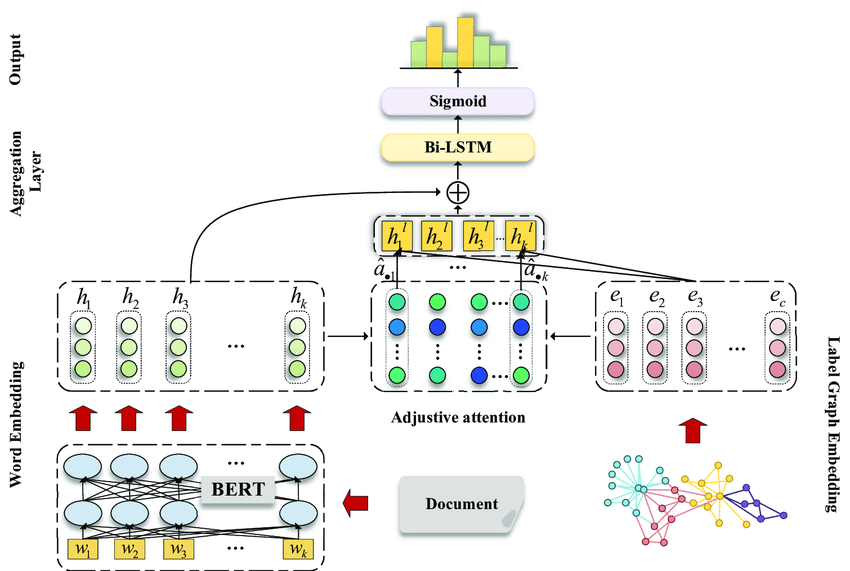
\includegraphics[width=0.6\textwidth]{figures/hbla_model.png}
  \caption{HBLA model~\parencite{cai2020hbla}.}
  \label{fig:hbla_model}
\end{figure}

In the domain of MLTC, the hybrid BERT model that incorporates label semantics via adaptive attention (HBLA), introduced by \textcite{cai2020hbla}, shows an advanced approach to addressing label dependencies. 
HBLA can simultaneously model a document and a label and obtain the hybrid word representation by an innovative adjustive attention mechanism that calculates the semantic relationships between words and labels.
It uses a graph convolutional network to capture label correlations through a label graph constructed from adjacency-based similarity as shown in Figure~\ref{fig:hbla_model}.

\begin{figure}[h!]
  \centering
  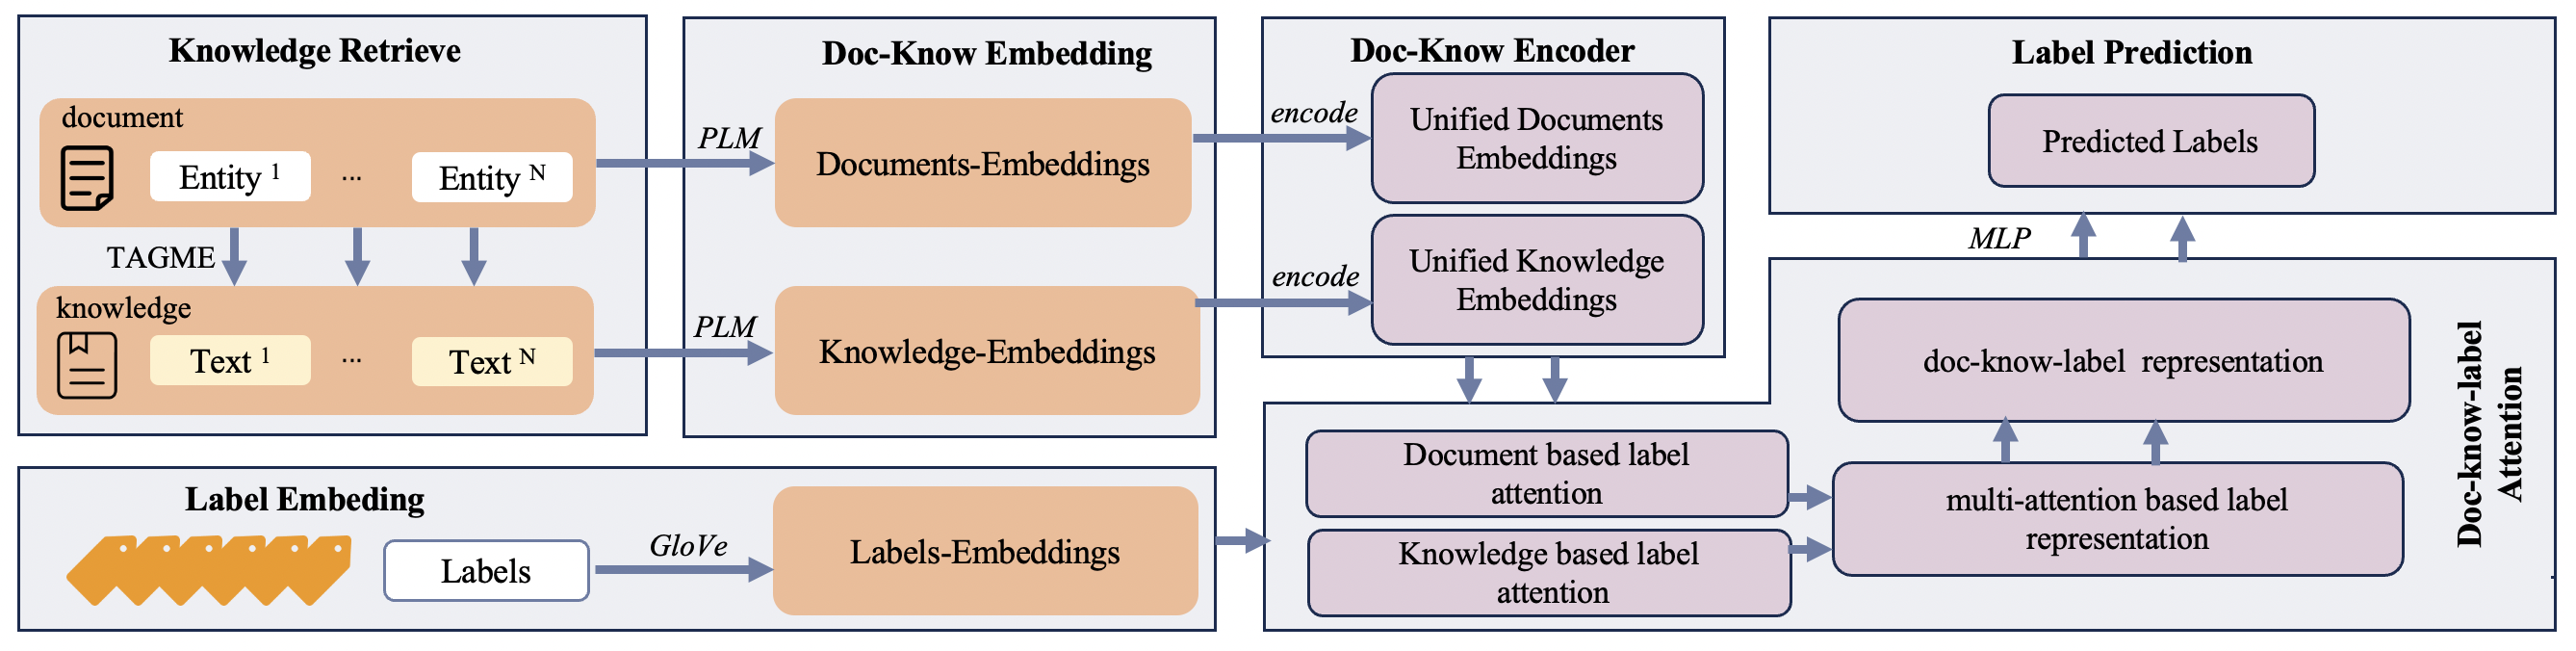
\includegraphics[width=0.9\textwidth]{figures/kenet_model.png}
  \caption{KeNet model~\parencite{li2024kenet}.}
  \label{fig:kenet_model}
\end{figure}

\textcite{li2024kenet} introduced the KeNet model, which demonstrates a retrieval-enhanced approach, utilizing knowledge retrieved from Wikipedia along with document embeddings. 
Both are processed using the same BERT encoder, while label embeddings are created using a GloVe~\parencite{pennington2014glove} encoder. 
These components are integrated through a Document-Knowledge-Label attention mechanism. 
This mechanism combines weighted attention between document-label and knowledge-label and effectively fuses information across documents, external knowledge, and labels to enhance data processing and interpretation.
Both MLTC methods presented above use BCE loss and sigmoid activation function for classification.

%--------------------------------------------------------------------------------------------------
% 
\chapter{Data Description}
\label{ch:data}
%--------------------------------------------------------------------------------------------------
Write introduction

\section{Data Preparation}

The dataset we used in our experiments comprises news articles labelled by the news monitoring industry, which tracks news outlets across six Central European and Western Balkan countries.

\begin{table}[h!]
\centering
\caption{List of Selected Industries}
\label{tab:industries}
\centering
    \resizebox{0.4\textwidth}{!}{%
        \begin{tabular}{l}
            Manufacturing \\
            Information and Communication Technology \\
            Healthcare and Pharmaceutical\\
            Finance and Insurance\\
            Foods and Agriculture\\
            Energy\\
            Retail\\
            Transportation\\
            Media and Entertainment\\
            Politics and Religion\\
            Automotive\\
		\end{tabular}
}
\end{table}

To obtain as diverse a representation of news media language as possible, we sampled the articles from January 2023 until December 2023, using labels corresponding to different industries monitoring news (see Table~\ref{tab:industries}). 
This sampled $NewsMon$ dataset comprises one million articles from eight countries (Serbia, Slovenia, Bosnia and Herzegovina, Croatia, Macedonia, Montenegro, Kosovo, and Albania) in more than seven languages (see Figure~\ref{fig:languages_hist}).
It is annotated with more than twelve thousand distinct labels. 
It encompasses all labels, not just the "seed" labels from the selected industries used for the initial selection.

\begin{figure}[h!]
  \centering
  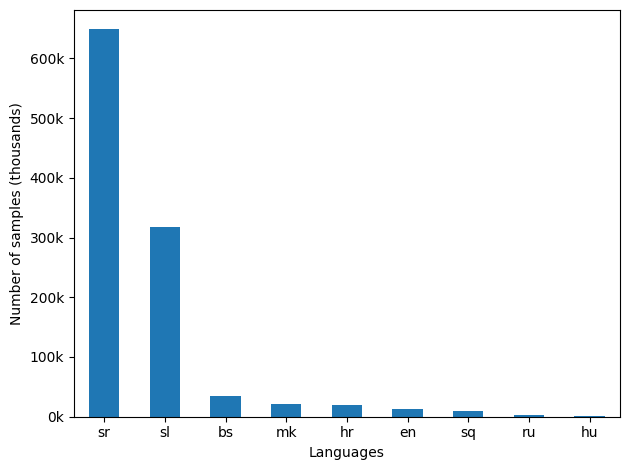
\includegraphics[width=0.5\textwidth]{figures/languages_hist.png}
  \caption{The distribution of languages across all samples (Serbian, Slovene, Bosnian, Macedonian, Croatian, English, Albanian, Russian and Hungarian).}
  \label{fig:languages_hist}
\end{figure}

Each article is assigned labels representing concepts or topics of interest to end-users.
Despite the system's vast number of labels, each end-user typically monitors only a few.
Each label is associated with several simplified Keyword-Boolean Expressions (KwEs) that determine the initial assignment of labels to news articles. 
News articles are automatically labelled based on those KwEs in the intake processing pipeline. 
At the final stage of the intake processing pipeline, a human moderator reviews the labels assigned to each article, as illustrated in Figure~\ref{fig:monitoring_flow}.
The moderator may confirm, reject, or add additional labels based on their assessment.
Labels and their corresponding KwEs are updated whenever a new user joins or leaves or when end-user interests change.
These updates can occur frequently, averaging about one hundred monthly label changes.
Arbitrary labels are also added at later stages by the analysis department.

\begin{figure}[h!]
  \centering
  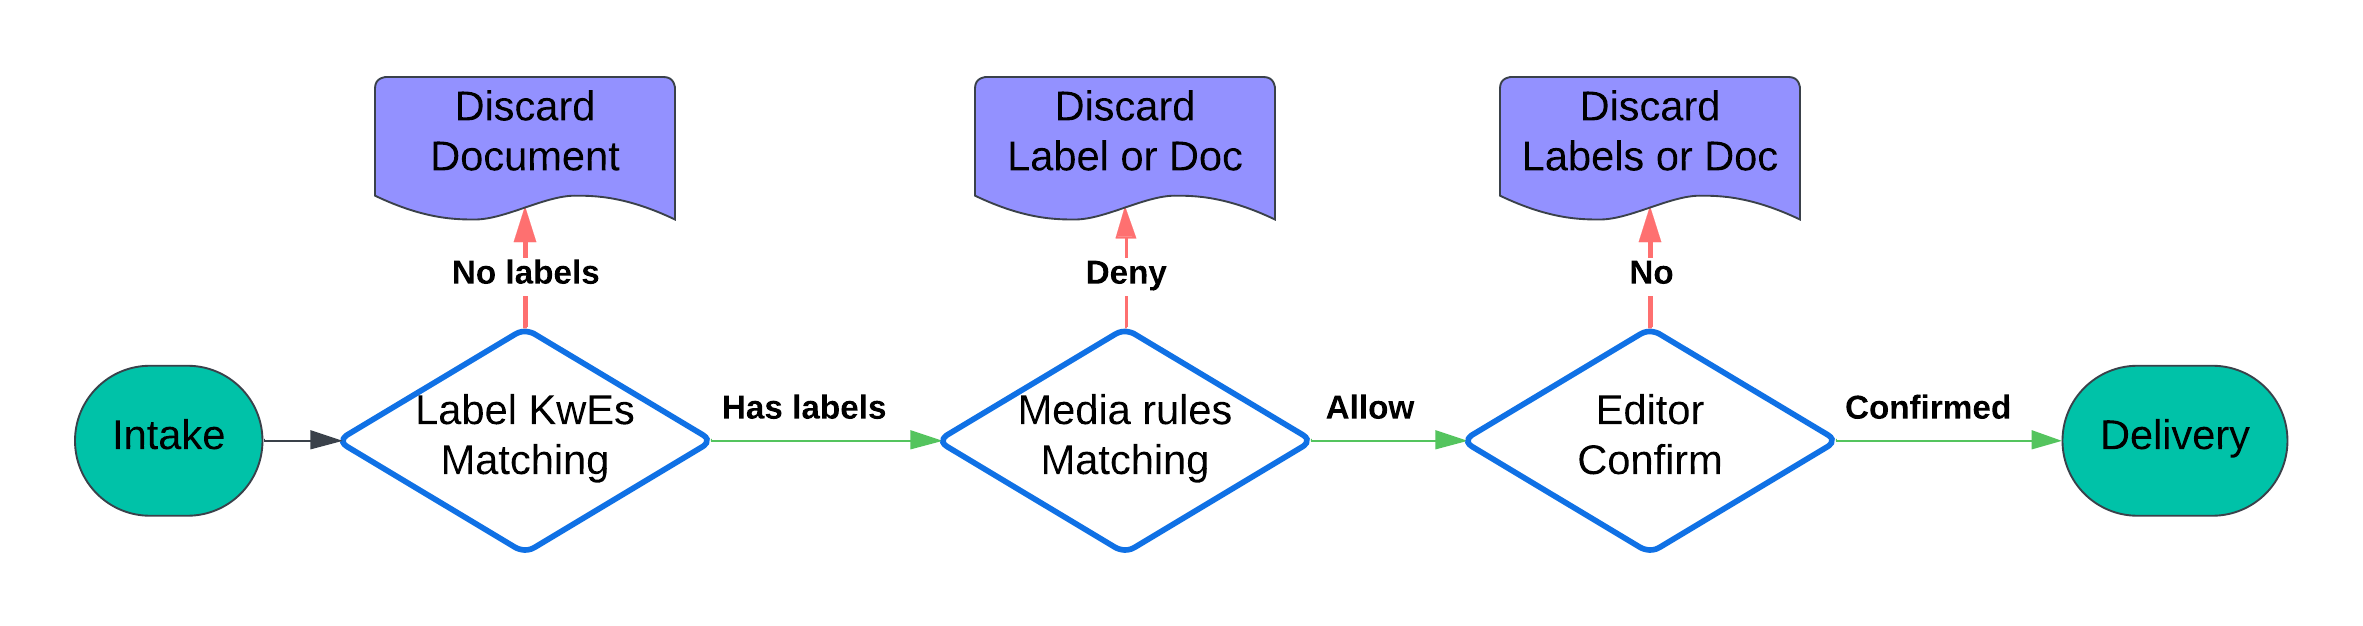
\includegraphics[width=0.9\textwidth]{figures/monitoring_flow.png}
  \caption{News monitoring intake processing pipeline.}
  \label{fig:monitoring_flow}
\end{figure}

\renewcommand{\arraystretch}{1.5}
\begin{table}[htb]
    \caption{Examples of simplified Keyword-Boolean Expressions}
	\label{tab:frames}
	\centering
    \resizebox{\textwidth}{!}{%
		\begin{tabular}{l|l}
            \hline
            \textbf{Keyword Expression}& \textbf{Explanation}\\
            \hline
            \hline
            \textbf{tesla OR teslo OR tesli OR tesle -"nikol* tesl*"}& Match the Tesla car brand if Nikola Tesla the person is not present in text\\
            \hline
            \textbf{mercedes* -formul* -"max verstap*" -F1 ...}& Match the Mercedes car brand if Formula 1 terms are absent.\\
            \hline
            \textbf{nlb* -"lig* nlb" -"nlb lig*"}& Match all forms of NLB terms, but only if NLB-sponsored league is not present.\\
            \hline
            \textbf{gradnj* -cest* -avtocest* -obvoznic*}& Match the term construction without the terms: road, highway or ring road\\
            \hline
            \textbf{\foreignlanguage{russian}{"сенад* софтић*"} OR "senad* softić*"}& Match the person with various inflections and in various scripts\\
            \hline
		\end{tabular}
  }
\end{table}
In the second iteration of data gathering, we collected the KwEs from moderator-confirmed labels along with their re-matched text spans.
Re-matched text spans provide an opportunity to pinpoint relevant text for specific labels, which could help address the issue of text truncation in specific targeted Transformer models and give us an opportunity for an effective information retrieval approach. 
Unfortunately, some labels still exist without their KwEs directly occurring in the text.
Upon further examination, we observed that the labels fall into two broad classes:
\begin{itemize}
  \item \textbf{Named Entities (NE)}: mostly Persons, Organizations, Products, Brands and rarely Locations.
  \item \textbf{General Concepts (GC)}: a set of terms representing a concept, for example, E-Mobility, Health insurance, Climate Change, Industrial waste.
\end{itemize}
We also found numerous labels with KwEs, most often from the NE class, that would match the same text.
These duplicates could potentially be removed, or the classification process optimized for the NE class of labels.
Some labels, especially from the GC class, are often context-dependent. 
For example, while the "Competition" label applies to many industries and seems like a duplicate, its meaning and KwEs vary depending on the context.
We further removed titles from the news article body text where present and combined them with the title to obtain a complete text.

\section{Data Analysis}

Due to the large dataset and label set size, we decided to down-sample the $NewsMon$ data, obtaining the $NewsMon_{sl}$ to speed up our research cycle for testing different classification methods and techniques.
We focused on publicly available Slovene data from January 2023 to May 2023, aiming for a dataset size and label distribution similar to other well-known multi-label datasets.
Next, we removed the labels that appear only once to prepare the $NewsMon_{sl+cls}$ dataset for baseline classifier training.
Below are some of the most popular datasets used for multi-label text classification we considered for comparison~\parencite{li2022surveytextclassification, tarekegn2024deeplearningmultilabellearning}:
\begin{itemize}
\item \textbf{Reuters-21578}: 
This widely-used dataset is derived from Reuters financial news services. 
It includes 90 classes containing 7,769 training texts and 3,019 testing texts (ApteMod corpus) containing single and multiple labels. 
Variants include subsets like R8 and BR52~\parencite{lewis1997reuters}.
\item \textbf{RCV1}, \textbf{RCV1-v2}, and \textbf{RCV1-2K}:
The Reuters Corpus Volume I (RCV1) comprises articles from Reuters News in 23 languages, collected between 1996 and 1997. 
It has 103 categories, featuring 23,149 training texts and 784,446 testing texts. RCV1-v2 includes corrections to the original dataset, while RCV1-2K expands the label set to 2,456 labels~\parencite{lewis2004rcv1}. With neural network approaches, test and train sets are usually swapped.
\item \textbf{AAPD (Arxiv Academic Paper Dataset)}: AAPD contains 55,840 academic papers from the Arxiv website, with abstracts and corresponding subjects labelled with 54 categories~\parencite{clement2019arxiv}.
\item \textbf{EURLEX57K}: EURLEX57K consists of 57,000 legislative documents from EUR-LEX. 
Each document is organized into four sections: the header (title and legal body), recitals (legal background), main body (usually articles), and attachments (e.g., appendices, annexes). 
The documents are annotated with concepts from EUROVOC, which includes around 7,000 labels. However, only 4,271 (59.31\%) of these are present in EURLEX57K, and just 2,049 (47.97\%) have been assigned to more than 10 documents.~\parencite{chalkidis-etal-2019-large}.
\item \textbf{AmazonCat-13K}: AmazonCat-13K is a large-scale multi-label text classification dataset commonly used for benchmarking extreme multi-label classification algorithms. The dataset consists of product titles and descriptions from Amazon. It contains 1,186,239 training samples and 306,782 test samples with 13,330 possible labels/categories. The average number of labels per sample is 5.04~\parencite{mcauley2013hidden}.
\end{itemize}

We specifically chose to compare our dataset with the $EURLEX57K$ dataset, a large-scale multi-label text classification (LMTC) dataset with properties similar to our down-sampled version regarding the label and instance size.
More importantly, comparing our dataset to the $EURLEX57K$ dataset allows us to evaluate the performance of our baseline classifiers in Chapter~\ref{ch:retrieval}.
We used $EURLEX57K$ model evaluation metrics to assess how well the same baseline model performs when trained on our dataset, considering our datasets consist of a lesser-used language in the model pretraining.
To do so, we first introduce label distribution metrics and then analyze the similarities and differences between the two datasets.

\subsection{Label Distribution Metrics}
To compare the datasets, we employed common label distribution metrics~\parencite{TAREKEGN2021107965, Bernardini2014CardinalityAD}.
We define Label Cardinality as the average number of labels per sample:
\begin{equation}
\text{Card}(M) = \frac{1}{m} \sum_{i=1}^{m} |Y_i|
\end{equation}
Label Density as the average number of labels per instance divided by the total number of  labels:
\begin{equation}
\text{Dens}(M) = \frac{1}{m} \sum_{i=1}^{m} \frac{|Y_i|}{|L|}
\end{equation}
and finally, Label Diversity as a number of distinct label combinations in the sample set:
\begin{equation}
\text{Diver}(M) = |{Y_x \subseteq L: (x, Y_x) \in M}|
\end{equation}
Where $M$ is the multi-label dataset, $m$ is the number of instances in $M$ (i.e., $m = |M|$), $Y_i$ is the set of labels for the $i$-th instance, and $L$ is the set of all possible labels in the dataset.

\subsection{Comparison}

All three datasets $NewsMon_{sl}$, $NewsMon_{sl+cls}$, and $EURLEX57K$ exhibit a long-tail label distribution, where most labels occur infrequently. 
They contain a large number of instances (ranging from 57,000 to 62,049) and a diverse set of labels (from 3,339 to 4,271).

\begin{table}[h]
    \centering
    \begin{tabular}{lrrrrr}
        \hline
        \textbf{Dataset} & \textbf{Samples} & \textbf{Labels} & \textbf{Cardinality} & \textbf{Density} & \textbf{Diversity} \\
        \hline
        \hline
        $NewsMon$ & 1,068,261 & 12,305 & 3.392 ± 4.017 & 0.00028 & 267,564 \\
        $NewsMon_{seed}$ & 1,068,261 & 1,960 & 2.213 ± 2.316 & 0.00114 & 183,361 \\
        $NewsMon_{sl}$ & 62,049 & 4,052 & 3.034 ± 3.492 & 0.00075 & 17,307 \\
        $NewsMon_{sl+cls}$& 62,049 & 3,339 & 3.023 ± 3.470 & 0.00091 & 17,202 \\
        \hline
        $EURLEX57K$ & 57,000 & 4,271 & 5.069 ± 1.701 & 0.00119 & 34,982 \\
        \hline
    \end{tabular}
    \caption{Shows the dataset statistics for the complete set ($NewsMon$), selected seed-set of labels ($NewsMon_{seed}$), the down-sampled dataset in Slovene ($NewsMon_{sl}$), and the down-sampled dataset with single occurrence labels removed ($NewsMon_{sl+cls}$).}
    \label{tab:dataset_statistics}
\end{table}

The $NewsMon_{sl}$ dataset includes 62,049 instances and 4,052 labels, with an average of 3.034 labels per instance. 
The label density is 0.00075, indicating that labels are distributed sparsely across the dataset.
The derived $NewsMon_{sl+cls}$ dataset also consists of 62,049 instances but with 3,339 labels, as single-occurrence labels were removed during filtering. 
Since we removed single occurring labels, the result is unsurprisingly a slightly lower average of 3.023 labels per instance but a higher label density of 0.00091, reflecting a more concentrated label distribution after filtering (see Table~\ref{tab:dataset_statistics}).

\begin{figure}[h!]
  \centering
  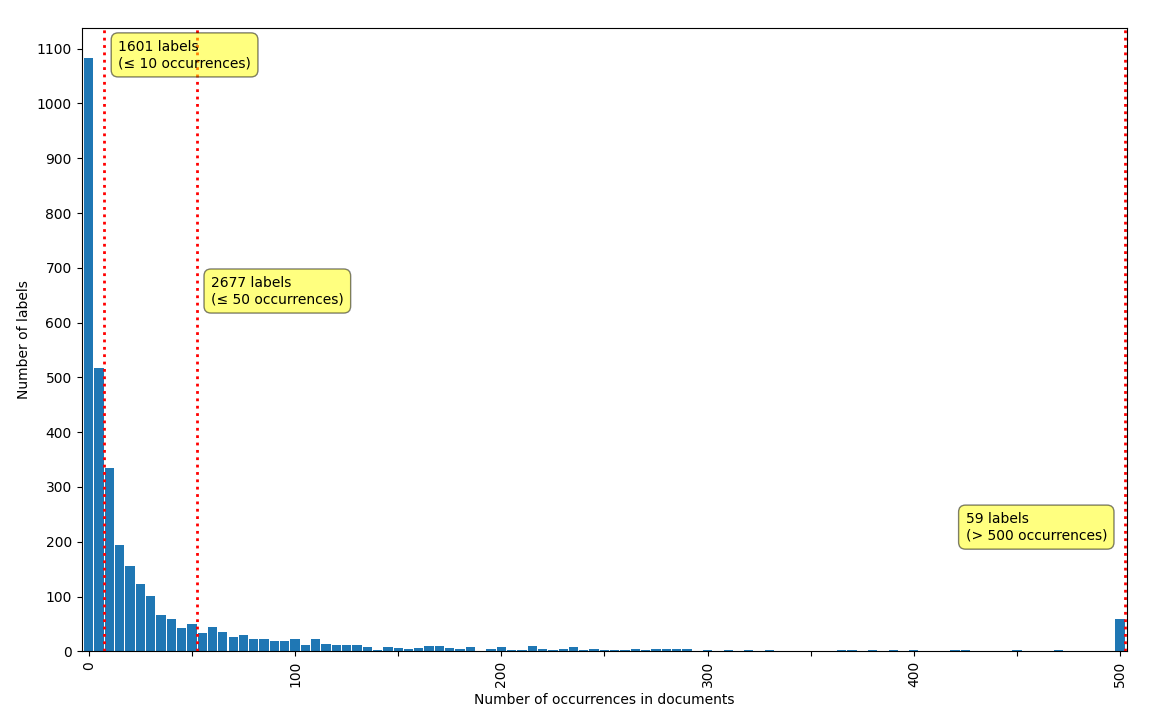
\includegraphics[width=0.8\textwidth]{figures/filtered_articles.png}
  \caption{The distribution of label occurrences in the $NewsMon_{sl+cls}$ dataset.}
  \label{fig:filtered_articles}
\end{figure}

\begin{figure}[h!]
  \centering
  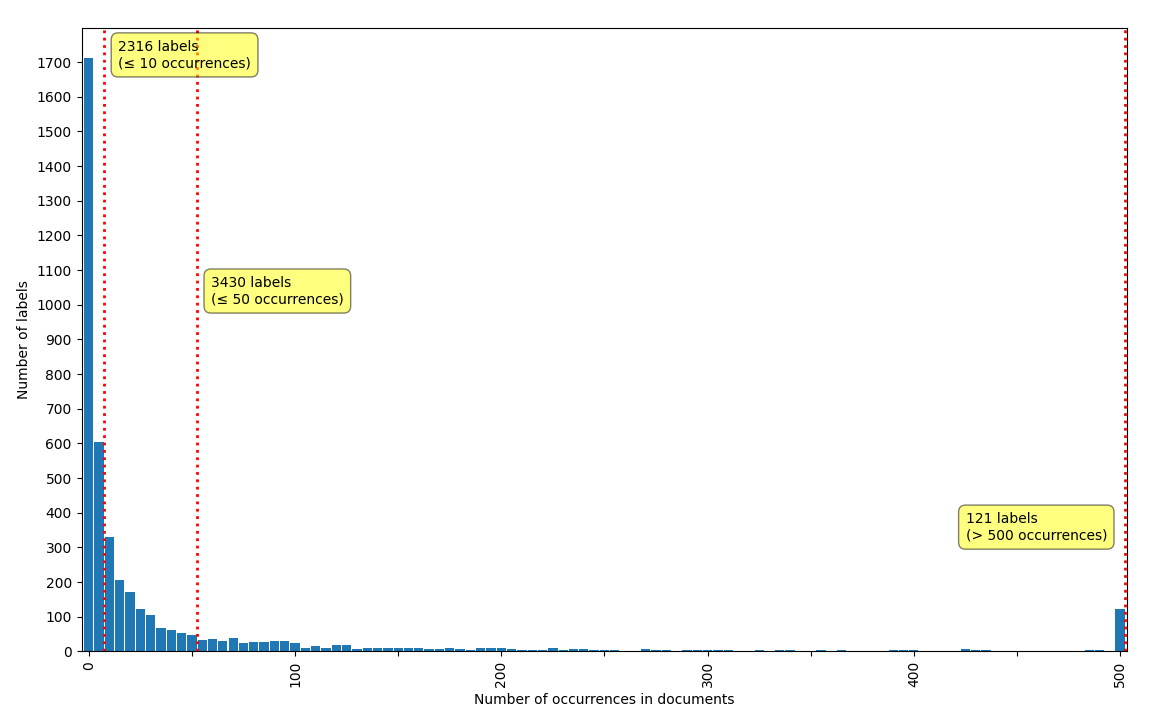
\includegraphics[width=0.8\textwidth]{figures/eurlex.png}
  \caption{The distribution of label occurrences in the $EURLEX57K$ dataset.}
  \label{fig:eurlex}
\end{figure}

The $EURLEX57K$ dataset, with 57,000 instances and 4,271 labels, has an average of 5.069 labels per instance and a label density of 0.00119, indicating a denser and more complex label distribution compared to the $NewsMon_{sl}$ datasets. 
This highlights the intricate label structure of $EURLEX57K$, while the $NewsMon_{sl+cls}$ dataset, after removing single-occurrence labels, shows a more concentrated label distribution than the unfiltered $NewsMon_{sl}$ dataset. 
A high standard deviation for cardinality in $NewsMon_{sl}$ datasets suggests that the number of labels per instance is spread out over a wider range.
Overall, the datasets show similar properties regarding the long-tail label distribution, which can be observed in Figure~\ref{fig:filtered_articles} and in Figure~\ref{fig:eurlex}.

%--------------------------------------------------------------------------------------------------
% 
\chapter{Retrieval Augmented Approach}
\label{ch:retrieval}

%In the next chapter,\todo{you mean this chapter (4)? or the next one (5)? Would be simpler and less ambiguous to say, "This chapter outlines our proposed method [\ldots]"} we will outline our proposed method, which uses an information retrieval (IR) approach to a large-scale multi-label classification problem to address the challenges of multilinguality, rare languages, low-resource environments, long-tailed label distributions, text truncation, and frequent label changes.

%We will start by introducing the selected baseline model and comparing it against baselines of models fine-tuned on a well-known and comparable $EURLEX57K$ dataset presented in Chapter~\ref{ch:data}. 
%This will be followed by discussing the embedding models we plan to employ. 
%Finally, we will present and discuss our proposed method and share preliminary zero-shot results.

In this chapter, we will first outline our proposed method, which uses an information retrieval (IR) approach to a large-scale multi-label classification problem.
This will be followed by a discussion of the embedding models we plan to employ. 
We will continue by introducing the selected baseline model and comparing it against baselines of models fine-tuned on a well-known and comparable $EURLEX57K$ dataset presented in Chapter~\ref{ch:data}. 
Finally, we will present and discuss zero-shot experiments and share preliminary results.

\section{Introduction}

In contrast to most models in XMTC and MLTC, which use end-to-end neural network training, our approach handles the classification and information retrieval tasks separately.
With this approach, we aim to address the challenges of multilinguality, rare languages, low-resource environments, long-tailed label distributions, text truncation, and frequent label changes.
%  in this initial research phase

\begin{figure}[h!]
  \centering
  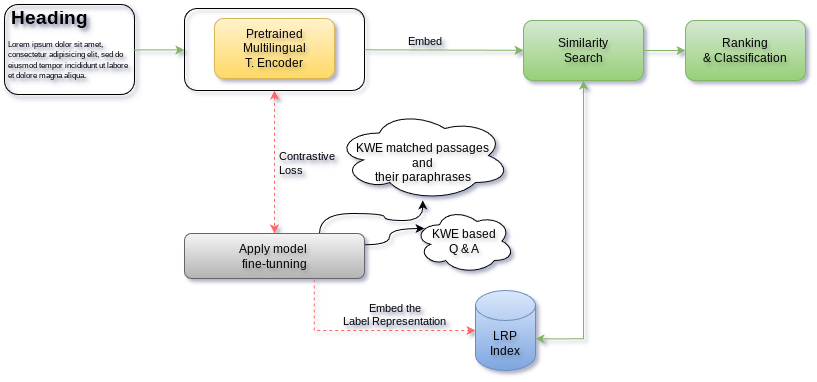
\includegraphics[width=1\textwidth]{figures/newsmon_model.png}
  \caption{The proposed framework: After model fine-tuning, we store label-relevant passages (LRP) together with label information in the LRP index (red line). 
  At inference time (green line), we search for similar passages, rank the search results, extract the label information and classify.}
  \label{fig:newsmon_model}
\end{figure}

We propose a straightforward approach that utilizes the pre-trained embedding IR model to encode both documents and label-relevant text passages (LRP).
During inference, the document is embedded as a query using the encoder and the LRP index is searched to retrieve all relevant labels.
For the classification task, we use the ranked top N similarity search results from the encoded LRP index based on an LRP-calibrated similarity threshold. 
To build an LRP index, we map each label with every encoded LRP for a particular label.
From the LRP, corresponding labels are mapped, and the IR ranking score is interpreted as classification probability, where only the highest score for each duplicate label match is considered~\ref{fig:newsmon_model}.
We opted to evaluate our method using a zero-shot approach for initial testing, meaning we did not fine-tune the IR model for the preliminary research.
For the zero-shot approach, we carry out similarity threshold calibration on the validation set to determine a per-label and overall average global similarity threshold, at which point classification for a given label becomes positive. 

We used re-matched text spans (MTS) on the $NewsMon$ dataset to identify text locations corresponding to specific labels for encoding LRP representations. 
We extracted different text context sizes based on sentence segmentation to form an LRP.
This extracted dataset will be our foundation for the model fine-tuning, which requires positive and negative query-passage pairs.
The best performance is achieved if the negative instances are similar but lack the target label—hard negatives (HN).
For mining the HN instances (those that are similar but lack the target label) from our dataset, we can use either a non-fine-tuned model, a competitive model~\parencite{wang2024multilinguale5textembeddings, xiao2024cpackpackagedresourcesadvance}, or the BM25 search algorithm.

\section{The Embedding Model}
For the document and LRP embeddings, we focused particularly on the M3-Embedding model (BGE-M3), noted for its adaptability across Multi-Linguality, Multi-Functionality, and Multi-Granularity~\parencite{chen2024bgem3embeddingmultilingualmultifunctionality}. 
The BGE-M3 model supports the semantic retrieval of over 100 operational languages. 
Additionally, it can simultaneously perform the three prevalent retrieval functionalities: dense retrieval, multi-vector retrieval, and sparse retrieval. 
Moreover, it can process inputs of varying lengths, ranging from sentences to documents containing as many as 8,192 tokens.
Considering its size and multilingual capabilities, the model achieves state-of-the-art performance on the MTEB~\parencite{muennighoff2022mteb} and Miracl~\parencite{zhang2023miracl} information retrieval benchmarks.

BGE-M3 is trained in two stages.
First, the XLM-RoBERTa model modified by the RetroMAE~\parencite{xiao2022retromae} is pre-trained using extensive unsupervised data, where only dense retrieval undergoes training using a basic form of contrastive learning. 
In the second stage, self-knowledge distillation is employed, fine-tuning the embedding model to refine the three retrieval functionalities.
Namely, it computes a weighted combined Noise-Contrastive Estimation loss (InfoNCE), introduced by \textcite{oord2019representationlearningcontrastivepredictive}, for each of the three functionalities.
Given that the $NewsMon$ dataset contains numerous named entities, the sparse retrieval, which compares token similarities between an encoded query and a text passage, can benefit our task.

\section{The Baseline Experiments}

To evaluate our method, we fine-tuned the multilingual pre-trained language model (PLM) and used it as a baseline classifier.
Namely, we selected XLM-RoBERTa-base~\parencite{conneau2019xlmr} from Huggingface~\parencite{wolf-etal-2020-transformers} and fine-tuned it on a $NewsMon_{sl+cls}$ using a Binary cross-entropy loss. 
Our previous research observed that the XLM-RoBERTa-base (XLM-R) model consistently outperforms the multilingual BERT~\parencite{ivacic2024comparing}. 
This is also the model from which the targeted embedding models were initially derived~\parencite{chen2024bgem3embeddingmultilingualmultifunctionality, wang2024multilinguale5textembeddings}.

We eliminated labels that appear only once to fine-tune the baseline model and conducted uniform random sampling to divide the $NewsMon_{sl+cls}$ dataset into an 80/10/10 split for the train, validation, and test sets, respectively. 
The labels in the $NewsMon_{sl+cls}$ dataset occur only once because of the removal of OCR, transcripts, and other non-publicly available data, as well as because the data was sampled only for selected labels and for a limited period.

For the baseline model training, we did not perform hyper-parameter optimisation; all the models are fine-tuned using the default set of hyper-parameters in the Transformers library, optimised for a large selection of common NLP tasks.
More precisely, following the methodology of \textcite{park2022efficient, chalkidis-etal-2019-large} we used similar settings as for $EURLEX57K$ dataset:
\begin{itemize}\itemsep=0pt
  \item AdamW optimiser with a learning rate of $3e-05$.
  \item Weight decay set to 0.01 for regularisation.
  \item Training for a maximum of 30 epochs.
  \item Batch size of 16.
  \item Dropout rate of 0.1.
  \item Maximum length of 512 sub-word tokens.
  \item Best model selection based on the validation set micro F1-score.
\end{itemize}
Based on initial test runs, we increased the maximum number of epochs from 20 to 30. 
We observed that learning stopped improving near the epoch 30.
Additionally, we increased the batch size to 16 to speed up training.
We repeated the fine-tuning process five times, setting a different random seed and re-shuffling the training set.

To evaluate the performance and, more importantly, to verify the implementation of our baseline classifier, we also fine-tuned the same PLM with the $EURLEX57K$ dataset.
All previous research reported evaluation metrics on the $EURLEX57K$ dataset model fine-tuned on a monolingual BERT; therefore, we couldn't compare directly with reported results.
%\todo{somewhere in this section, maybe worth saying that the "baseline" is more computationally expensive (I guess?) and involves more annotated data than your proposed approach}
% TODO: check this ... media outlet rules might influence rare label frequency.

To assess the feasibility of our approach with the selected BGE-M3 model, we conducted an additional zero-shot baseline experiment using the simplest method possible. 
For this experiment, we first embedded the training set and stored these embeddings in an index, along with their corresponding labels. 
Next, we chose samples from the test set, using their labels as ground truth for the classification task. 
Finally, we performed a cosine similarity search for each test sample and assigned labels from the closest training instance as predictions. 
We did not fine-tune the model, utilize label-relevant passages, or implement any ranking system.
Additionally, we didn't search at which threshold the similarity search yields the best classification results.

\clearpage 

\begin{table}[h]
    \centering
    \resizebox{\textwidth}{!}{%
        \begin{tabular}{lccccccc}
        \hline
        \textbf{Model} & \textbf{Corpus} & \textbf{Micro F1} & \textbf{Micro P} & \textbf{Micro R} & k & \textbf{R-Precision@k} & \textbf{NDCG@k} \\
        \hline
        BERT & $EURLEX57K$ & \textbf{73.2}  & - & - & 5 & \textbf{79.6} & \textbf{82.3}  \\
        XLM-R & $EURLEX57K$ & 68.765 $\pm$ 0.182 & 85.086 $\pm$ 0.318 & 57.698 $\pm$ 0.246 & 5 & 76.256 $\pm$ 0.218 & 79.200 $\pm$ 0.193 \\
        \hline
        XLM-R & $NewsMon_{sl+cls}$ & 61.559 $\pm$ 2.306 & \textbf{85.952} $\pm$ 0.408 & 47.988 $\pm$ 2.710 & 3 & 79.649 $\pm$ 1.740 & 80.084 $\pm$ 1.819 \\
        BGE-M3 & $NewsMon_{sl+cls}$ & \textbf{66.151} & 65.259 & \textbf{67.067} & - & - & - \\
        \hline
        \end{tabular}
    }
    \caption{Baseline XLM-R classifier performance metrics for $EURLEX57K$ and $NewsMon_{sl+cls}$ corpora. For BERT PLM, we show metrics reported by \textcite{chalkidis-etal-2019-large}; for the XLM-R model, we show our baseline classifier metrics. We report at K = corpus label cardinality~\parencite{chalkidis-etal-2019-large}.}
\label{tab:baseline_metrics}
\end{table}

The evaluation results of the baseline classifier on the test set are presented in Table~\ref{tab:baseline_metrics}.
If we first compare conventional PLM models, we can see that the performance dropped noticeably when using a multilingual model for $EURLEX57K$ text. 
Observing the standard deviation with micro-averaged F1 and recall, we can see that training the baseline classifier on a $EURLEX57K$ dataset has much more predictive results compared to $NewsMon_{sl+cls}$. 
$NewsMon_{sl+cls}$ fine-tuned baseline classifier has a significantly worse recall, indicating that the model struggles to identify all the relevant labels for each instance. 
Since the precision of the two models is close, we can assume that the $NewsMon_{sl+cls}$ model has a higher rate of false negatives compared to the $EURLEX57K$ model.

Next, comparing a simple similarity search with conventional PLM, we can observe that similarity search combined with BGE-M3 embeddings outperforms the XLM-R baseline classifier on micro F1 score by improving overall recall.
Consequently, we can view the XLM-R model as being more precise but considerably more conservative, favouring false negatives over false positives. 

We noticed duplication phenomena in the dataset when we analysed the individual classification samples for the zero-shot experiment.
Some news articles were duplicated but appeared in different outlets or news aggregators. 
Some were very similar in content, for instance, a summary of the official press release or social media posts with picture changes that are not reflected in the content itself (see Table~\ref{tab:social_dup}).
We believe this is a significant factor in the performance of the simple similarity search. 
Further analysis would be necessary to confirm this.


\begin{table}[h]
    \centering
    \resizebox{\textwidth}{!}{%
        \begin{tabular}{l}
        \hline
        \makecell{
        [IMAGE]: River Krka in Novo mesto, S... \\
\\
River Krka in Novo mesto, Slovenia \#visitdolenjska \#igdolenjska \#visitslovenia \#ifeelslovenia \#geoslovenija \#nasvetzaizlet \\ 
\#kampadanes \#ig\_brilliant \#special\_shots \#main\_vision \#discoverglobe \#ourplanetdaily \#earthofficial \#earthoutdoors \\ 
\#splendid\_view \#roamtheplanet \#stunning\_shots \#amazing\_shots \#theglobewanderer \#wanderlust \#travelphotography \\ 
\#travelgram \#traveladdict \#worldbestgram \#ig\_captures \#djimini3pro \#ig\_exyu \#beautifuldestinations \#nature \#naturephotograph
} \\
        \hline
        \end{tabular}
    }
    \caption{An example social media post from $NewsMon_{sl+cls}$ corpora which is repeated for every update.}
\label{tab:social_dup}
\end{table}

%--------------------------------------------------------------------------------------------------
% 
\chapter{Conclusion}
\label{ch:trends}
%--------------------------------------------------------------------------------------------------
This chapter provides a concise overview of key considerations for our method, followed by potential improvements to our previous research.

\section{General Considerations}

By separating the classification and encoding of dense document and label representations, we can solve the problem of frequent label changes since we do not need to retrain the model end-to-end when enough label changes accumulate. 
Every label can be updated or removed simply by altering the label-relevant text passage (LRP) index.
Additionally, if we separate these two components, we can more easily replace the embedding model when better-performance models emerge.
Since we do not fine-tune end-to-end, we lose classification performance but gain greater explainability. 
We can easily explain why the classifier selected a certain label based on the document's similarity to the LRP.
Finally, since the model is not fine-tuned end-to-end for the multi-label classification task, it could be employed for additional purposes, such as clustering, general retrieval and summarization.

\section{Future work}

Upon examining our work, several areas for potential improvements emerge. 
Initially, a more detailed data analysis could enhance classification accuracy. 
By analyzing the labels more deeply, we could determine the proportion of labels belonging to Named Entity (NE) classes versus those representing General Concepts (GC). 
Incorporating a supplementary Named Entity Recognition (NER) model~\parencite{ivacic2023analysis} would allow us to identify duplicates in label classes and NEs. 
This integration would enable us to tailor the classification type based on label class during inference.

Moreover, it is crucial to determine how many labels lack associated text spans, necessitating the synthesis of relevant label text passages. Employing techniques such as LLM prompting and paraphrasing can significantly improve information retrieval results~\parencite{wang2024improvingtextembeddingslarge}
Additionally, categorizing labels by frequency and analyzing performance across these categories (frequent, rare, etc.) could help pinpoint weaknesses in our classification framework and guide further improvements.

Finally, fine-tuning the model with query text passage pairs at different granularity should be tested.

\section{Summary}

We have explored multi-label text classification (MLTC) as applied to the news monitoring industry and discussed using advanced NLP technologies to address the identified challenges. 
Next, we discussed our approach to preparing and analyzing this multilingual and multi-label dataset, outlining the specific challenges and the strategies we employed.
We reviewed MTLC evaluation metrics used in research together with contemporary methods, followed by problems with representing lengthy documents. 
We further discussed transitioning from conventional MLTC methods to more intricate scenarios requiring different approaches and advanced handling techniques for large-scale datasets.
We presented a retrieval-augmented approach tailored to address specific challenges such as multilinguality, rare languages, and frequent label changes. 
This approach benefits low-resource languages and systems, which often suffer from a scarcity of training data and unusable models.
Leveraging these emerging paradigms, we plan to continue our research, focusing on applied solutions for news analysis.
We have laid the groundwork for advancing the application of NLP technologies in news monitoring, addressing the pressing challenges through innovative methodologies.
%--------------------------------------------------------------------------------------------------
%
% APPENDICES (optional)
%--------------------------------------------------------------------------------------------------
%
\appendix
\begin{appendices}
%
\end{appendices}
%--------------------------------------------------------------------------------------------------
%
% BACK MATTER
%--------------------------------------------------------------------------------------------------
%
\backmatter
%
% References used in the thesis
\printreferences
% 
% Author's bibliography 
%%--------------------------------------------------------------------------------------------------
% 
\chapter{Bibliography}
%--------------------------------------------------------------------------------------------------
% Enclose with refsection and use \nocite{*}, if you need to list publications not referenced in 
% the thesis:
\begin{refsection}
\nocite{*}

\section*{Publications Related to the Thesis}

All publications related to the thesis should be referenced in the text.

\defbibheading{subbibliography}{\subsection*{Journal Articles}}
\printbibliography[heading=subbibliography,keyword=myarticle]

\defbibheading{subbibliography}{\subsection*{Conference Paper}}
\printbibliography[heading=subbibliography,keyword=myconf]

\section*{Other Publications (optional)}

\dots

\end{refsection}
%
% Author's biography
%\input{text/back-biography}
%
% Index (optional)
%\printmyindex
%--------------------------------------------------------------------------------------------------
\end{document}
%--------------------------------------------------------------------------------------------------
%
% MODIFICATION HISTORY
%--------------------------------------------------------------------------------------------------
% Version 1.3:
%  - Removed the sorting option from \printbibliography in IEEE bibliographies due to a new warning.
% Version 1.2: 
%  - Modified the symbols and abbreviations example to adjust the vertical positioning of the text
% Version 1.1: 
%  - Removed slovene.lbx and slovene-apa.lbx from accompanying files as they are now included in 
%    the latest biblatex version.
%  - Modified the bibliography example to include publications not referenced before.
%  - Modified the references example to show DOI should be used only for articles not yet published. 
%  - Modified the symbols and abbreviations example to accommodate long lines and long lists.
%  - Added pdf bookmarks for Acknowledgments, Abstract and Povzetek. 
%--------------------------------------------------------------------------------------------------
